\chapter{Introduction}
\section{Motivation}
It is estimated that there are nearly two million people living with limb loss in the United States \cite{ziegler-graham_estimating_2008}. Among those living with limb loss, the main causes are vascular disease (54\%) including diabetes and peripheral arterial disease trauma (45\%) and cancer (less than 2\%) \cite{ziegler-graham_estimating_2008}. Approximately 185,000 amputations occur in the United States each year \cite{owings_ambulatory_1998}. In 2009, hospital costs associated with amputation totaled more than \$8,3 billion \cite{varma_physical_2014}. In the work of Robbins et al. they estimated that nearly half of the individuals who have an amputation  will die within 5 years due to vascular disease. This is higher than the five-year mortality rates for breast cancer, colon cancer and prostate cancer \cite{robbins_mortality_2008}. Partial hand amputation with loss of one or more fingers, is the most prevalent upper limb amputation \cite{tenore_towards_2007}. Since hand and finger dexterity requires muscle in the forearm and since $\sim$70\% of all upper limb  amputations are distal to the elbow this makes the case for the development of hand prostheses with a high degree of dexterity \cite{dillingham_limb_2002,weir_persons_2000}. From the above mentioned we can conclude that the need for the development of prosthetics that can successfully translate the electrical signals from the nerves into the correct finger gesture motion is of great importance. In this work, we will propose a pipeline in order to show how to prepare these raw signals into meaningful input for the powerful artificial neural networks. \\  
Fingers are the most used limbs of the human body which help in sensing and manipulating objects. Moreover, finger motions enable humans to express our feelings. One can understand that the variety of finger gestures are endless as they are used from controlling physical objects to expressing intangible ideas. The possibility of employing algorithms to recognize this whole spectrum of finger motions can give an extensive insight into human's everyday life. The mobile devices are some of the physical objects that humans are carrying on them everyday while walking, running, or just waiting for the bus to come. By moving our fingers, we are able to control the user interface of these mobile devices by selecting, adding and deleting elements. Therefore, finger gesture recognition is also significant for human-computer interaction. \\
There are different kind of mobile devices such as smart watches, mixed-reality-glasses, mobile phones and tablets. Smart watches and glasses due to their small surface promote the idea of an immersive usage with micro-interactions as the usage of onscreen keyboards seems to be impossible. On the contrary, mobile phones and tablets due to their bigger screen have already replaced a great percent of computers. The increasing interest of consumers to control more with smaller, mobile devices gives the chance to wearable technology to emerge. Most of the wearables nowadays do not have keyboard or a wide screen so it is necessary to employ gesture recognition technology. Thus, the need for hands-free human-machine interfaces will help many disabled people who have difficulty to access assistive robotic systems and rehabilitation devices.\\
At present, there are various methods for capturing and recognizing finger gestures, such as video signal, image analysis, electromyography (EMG) \cite{zhang_tomo:_2015,shin_dynamic_2016,kakoty_exploring_2015,zhao_study_2007}. Many researchers tried to capture finger gestures with cameras but the poor lighting conditions leads to misclassifications. Moreover, the usage of sensing gloves as well as the utilization of capture motion techniques burden the labs with expensive equipment and cost of expertise personnel. Furthermore, most of the existing EMG gesture recognition techniques involve special sensors made for a certain lab that are not available in the science community and therefore experiments cannot be repeated accurately. In this work, the use of EMG signals acquired by the hand of the subjects will be used to detect finger gestures. Myo is a gesture control armband which can acquire among other data, EMG signals.\\
In the last decade, great progress was made in the area of gesture controlled devices. Nod \cite{nod}, Mycestro \cite{mycestro} and Myo \cite{myo} are some of the devices that made the major breakthrough in this industry. The aforementioned devices are successfully controlled with the user’s hand gestures thanks to the integrated sensors such as gyroscope, magnetometer, accelerometer and EMG sensors. Scientists soon came to realise that these devices can help not only in controlling basic remote control functionalities such as changing the volume and the brightness of the sound and video respectively, control basic video flow functionalities such as play, pause, rewind and forward and  navigate through different channels but also assist them in gathering data that will help them develop their own ideas and concepts on various fields. These techniques can be useful in designing human machine interfaces, control prosthetics and robots and help in rehabilitation for people with motor disorders. Myo is one of these wearable devices that opened new fields in research.\\
The aim of this work is to find the most accurate classifications between the different finger gestures. Firstly, we acquire the EMG signals and the video with the recorded finger movement from the cell phone. Then, we eliminate all possible artifacts which happen due to the variable frame rate of the cell phone's camera. After the elimination of the artifacts, we segment the total EMG signal to smaller parts which represent the candidate movements which will be classified, for example flexion and extension of the thumb. Then, the segmented data are separated into five folds for the training data with which we will train the classifiers and five folds for the testing data with which we will test the newly trained network and one evaluation fold. After the separation of the data, we will pre-process the raw data with root-mean-square (RMS), moving average (smooth), short-time fourier transform (STFT) and different discrete wavelet transforms (DWT). With the processed data, the classifiers are trained with each training fold and then tested with the corresponding test fold and the accuracies are calculated. The final outputs are tested with the evaluation fold. The most accurate features will help us to determine which training folds we will conjuct to re-train the network with them. \\
To sum up, the current work will add knowledge on how EMG signals coming from finger motion should be preprocessed and classified in order to get accurate classifications. This will give an insight on how the preprocessing of EMG signals can improve the accuracy and efficiency of muscle-controlled devices. This will enable people with motor disorders to better control exo-skeletons such as artificial fingers or arms in cooperation with wearable devices such as the Myo. Myo has the dynamic of an out-of-the box product which can be used as a potentially lower-cost alternative to other mind-controlled devices.\\

\section{State of the art}
Nymoen et al. developed a musical instrument prototype aimed to investigate the use of Myo armband with various instrumental actions \cite{nymoen_mumyoevaluating_2015}. Researchers at the Johns Hopkins University Applied Physics Laboratory  have already developed a new surgical technique that allows an amputee to control a modular prosthetic limb with two Myo armbands \cite{myo_arm}. Kutafina et al. proposed to use the Myo wearable armband to measure correctness of hand washing for mobile learning which is an important part of medical education \cite{kutafina_wearable_2015}. Yang  developed a method to tele-control a robot arm to imitate human writing skills using electromyography (EMG) signals which were acquired by the Myo armband \cite{yang2015teleoperated}. Dash et al. created a novel algorithm which converts the hand movements in the air into a sequence of 2D coordinates on a 2D plane\cite{dash_airscript-creating_2017}. Their approach provides a recognition module to predict the content of the document created in air. Their algorithm employs deep learning methods which uses the sensor data and the visualizations created by their algorithm. Kosmidou and Hadjileontiadis  analyzed EMG and IMU data with intrinsic-mode entropy to recognize Greek Sign Language (GSL) isolated signs\cite{kosmidou_sign_2009}. Cheng and Liu adopted a discrete wavelet transform (DWT) to analyze the acquired surface EMG signals to recognize successfully different emotions \cite{cheng_emotion_2008}. Ververidis et al. are researching features such as muscle total pressure, flexors pressure, tensors pressure and gesture stiffness for the purpose of identifying differences in performing the same gesture across different pottery constructions \cite{ververidis_pottery_2016}.\\ 
In all of the above work, the wrist motion of the hand such as the radial and ulnar deviation, wrist pronation/supination and wrist flexion/extension are extensively researched whereas the discrimination of the intention and the control of the fingers motion by surface EMG signals from a human arm still remains ambiguous. In this work, we will try to deepen our knowledge on detection of finger gestures, acquired from the arm of the subject with the EMG sensors of Myo armband. The uniqueness of this work is that  the results of this work will be based only on EMG signals coming from the muscles of the forearm, acquired by the Myo device, leaving \ac{IMU} data out of the equation. Focusing only on the motion of the fingers, there is no need to set the arm of our subject in motion, therefore we keep it still in a fixed position. Furthermore, the mobility of the Myo as it is wireless and connects to a PC or a mobile phone via Bluetooth connection can only be added to the advantages. Last but not least, Myo armband is the most economic solution for surface electromyography as it costs 170 euros while the cheapest portable electromyograph system costs around 4500 euros \cite{EMG_device_price}.\\

\section{Electromyography}
Electromyography is a method for recording the electrical activity produced by muscles. The electrical nerve impulses are transmitted from the brain to the muscles of the arm, which in this work we are studying, via the nervous system. To measure and quantify the electrical nerve impulses EMG has transeivers that help to transmit or receive these electrical impulses. Depending on where the sensor is placed we can conclude which muscles are contracted and how strong the contraction is.\\
There are two kinds of EMG sensors: the intramuscular Fig \ref{Fig:intramuscular_needle} and the surface EMG recording electrodes Fig \ref{Fig:surface_emg_electrodes} .
\begin{figure}[h!]
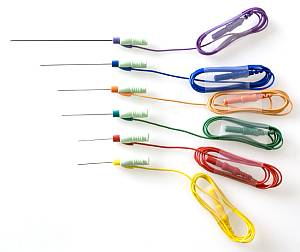
\includegraphics[width=10cm,center,keepaspectratio]{figures/intramuscular_needle}
\caption{Disposable Hypodermic Needle Electrodes\cite{Disposable_Hypodermic_Needle_Electrodes}}
\label{Fig:intramuscular_needle}
\end{figure}
\begin{figure}[h!]
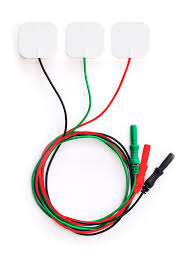
\includegraphics[width=7cm,center,keepaspectratio]{figures/surface_emg_electrodes}
\caption{EMG Surface Electrodes\cite{surface_emg_electrodes}}
\label{Fig:surface_emg_electrodes}
\end{figure}
With intramuscular electrodes we can track which exact muscle is contracting and can get a precise signal resolution from each muscle. The disadvantage is that the procedure is invasive which can become unpleasant for the patient. On the contrary, surface electrodes are placed on the patient's skin, in our case Myo's electrodes, to measure the electrical impulses and are non-invasive which means that they do not provoke any physical discomfort to the patient. The disadvantage is that they are restricted to superficial muscles which induces that it cannot track the electrical activity of one muscle but captures all signals from the muscles in the vicinity of the sensor. This phenomenon is also known as cross-talk \cite{winter_crosstalk_1994}. In the forearm there are many different muscles each in different distance from the surface electrode. If an adjacent muscle is active rather than the one directly below the electrode, a crosstalk signal can be detected and misinterpreted as originating from the muscle of interest. The resulting signal is an estimate of the overall muscular activity from the adjacent muscles. Another restriction of the surface electrodes, is that the final output signal is also influenced by the patient's traits such as percent of skin fat, hairiness and perspiration. Fatty skin tissue lead to distortion of the signal and hairiness hinders the contact between the sensor and the patient's skin.\\
\section{Stationary signals}
Before analyzing the reason EMG signals are non-stationary signals we will explain what  a stationary and a non-stationary signal is. A signal is stationary if its frequency is not changing with respect to time. When we generate a sine wave we determine the frequency and keep it constant. Ergo, the frequency of the sine wave is constant through time and hence this signal is an example of a stationary signal. Stationarity is linked with the behavior of the frequency and has nothing to do with the time varying amplitude of the wave \cite{sakshat_virtual_labs}. In Fig. \ref{Fig:singletone} we see a stationary signal which in this case is a sine wave. We observe that its frequency is constant whereas the amplitude varies. In the following figure we plot the equation $y = sin(2\pi10t)$.
\begin{figure}[H]
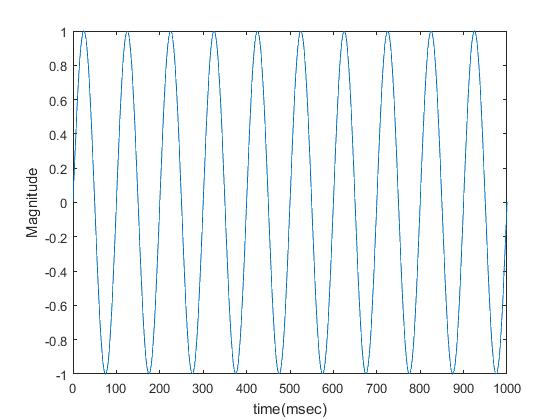
\includegraphics[width=12cm,height=10cm,center,keepaspectratio]{figures/singletone}
\caption{Sine wave of 10 Hz sampled using a sampling frequency of 1000 Hz.}
\label{Fig:singletone}
\end{figure}
A signal can be also stationary when even it has different frequencies, they do not change over time. If the frequencies of a multitone sine wave do not change over time, regardless of how many frequency components the wave is consisted of, then the signal is stationary. A multitone wave can be written as the Equation \ref{Eq:multitone_wave}:
\begin{equation}
y = A_1sin(\omega_1t + \phi_1) +A_2sin(\omega_2 t + \phi_2) +A_3sin(\omega_3 t + \phi_3)
\label{Eq:multitone_wave}
\end{equation}
Next, is the waveform of a multitone signal:
\begin{figure}[H]
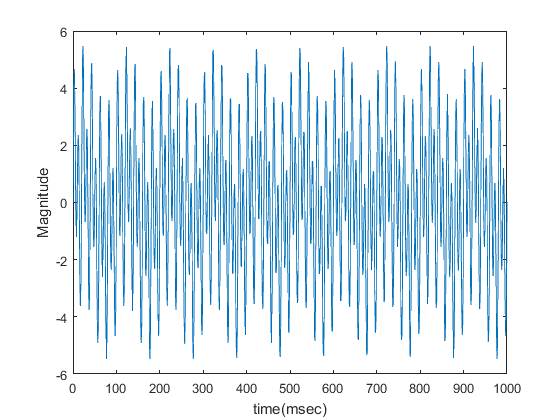
\includegraphics[width=12cm,height=10cm,center,keepaspectratio]{figures/multitone}
\caption{Multitone sine wave of 10, 50 and 100 Hz sampled using a sampling frequency of 1000 Hz.}
\label{Fig:multitone}
\end{figure}
Although, its waveform is more complicated than the previous one, it is a stationary signal as its frequencies remain constant through time.
\section{Non-stationary signals}
Let's assume a multitone signal whose duration is divided into four intervals. Let's assume frequency $f_1$ is present in the first interval, $f_1$ and $f_2$ in the second interval, $f_1$, $f_2$ and $f_3$ present in the third interval and $f_1$ in the fourth interval. We observe that the frequenies are changing from interval to interval. Thus, this wave qualifies as non-stationary. For example in Fig. \ref{Fig:non-stationary} we consider a non-stationary wave with frequency 10 Hz for the first interval, 10 and 50 Hz for the second interval, 10, 50 and 100 Hz for the third interval and 10 Hz for the fourth interval.
\begin{figure}[h!]
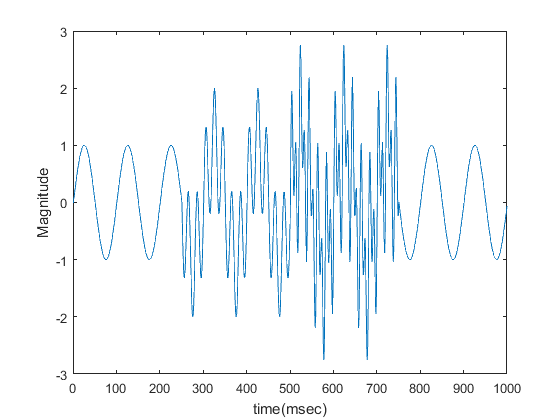
\includegraphics[width=15cm,left,keepaspectratio]{figures/non-stationary}
\caption{Non-stationary multitone sine wave of 10, 50 and 100 Hz sampled using a sampling frequency of 1000 Hz.}
\label{Fig:non-stationary}
\end{figure}
In Equation. \ref{Eq:non-stationary_wave} we give the mathematical formulation for such a signal. 
\begin{equation}
x(t) =
\begin{cases} A_1sin(\omega_1t + \phi_1) & 0 \leq t \leq t_1 \\
      A_1sin(\omega_1t + \phi_1) + A_2sin(\omega_2 t + \phi_2) & t_1 \leq t \leq t_2 \\
      A_1sin(\omega_1t + \phi_1) + A_2sin(\omega_2 t + \phi_2) +A_3sin(\omega_3 t + \phi_3) & t_2 \leq t \leq t_3 \\
      A_1sin(\omega_1t + \phi_1) & t_3 \leq t \leq t_4
\end{cases}
\label{Eq:non-stationary_wave}
\end{equation}
\subsection{Cause of non-stationarity in EMG signals}
During muscle contractions, joint angles various muscles work together in order to perform a certain movement. This may involve the recruitment or the de-recruitment of muscles for rapid contributions, which will introduce non-stationarities to the final EMG signal. Also, due to changes in the joint angles, the underlying muscles change position relative to the recording electrodes. This results in the electrodes not to be correctly positioned above the muscles and this affects sequentially the recorded frequency. Last but not least the variability of the length of the muscle fibers can influence as a scaling factor to the power spectrum of the EMG signal \cite{bonato_time-frequency_2001}. Furthermore, when the muscle is getting tired, metabolites are accumulated over time in the muscle. The metabolites result in a decrease of conduction velocity of the motor action along the muscle fibers. This affects the power spectrum of EMG signals and thus introduces non-stationarities in the EMG signal \cite{bonato_time-frequency_2001}. \\

\section{Thalmic Myo} 
Thalmic Myo shown in Fig. \ref{myo} was developed by Thalmic Labs in 2014 \cite{thalmic}. It is worn on the forearm and enables the user not only to control a computer as a computer mouse would do but also can provide the control of various gagdets such as quadocopters and gyroballs with the help of hand detection.  \\
Large parts of the Myo's software \cite{myo_developer} is publicly available and Thalmic labs provides access to development kits for most of the operating systems. Furthermore, they explain their ideas behind the implementation and help the developers to extend their product by adding more functionalities to it. \\
The Myo is extendable from 19 cm to 43 cm forearm circumference. The Myo armband is 1.1 cm thick and weights 93 grams. \\
As Myo is a wearable device, it is programmed to transfer the collected data to another device. Thalmic Myo uses Bluetooth connection as the communication protocol between the Myo and the client. The structure of Myo is equipped with eight stainless EMG sensors designed for recognizing hand gestures and movements. It also consists of a 9-axis (IMU) Inertial Measurement Unit used to detect arm movements. The IMU consists of a 3-axis gyroscope, a 3-axis accelerometer and a 3-axis magnetometer. \\ The accelerometer and gyroscope are basic common sensors that come with every mobile phone device and smart wearable devices such as fitness trackers. The novel approach of Myo is the embedded EMG sensors.
\begin{figure}[H]
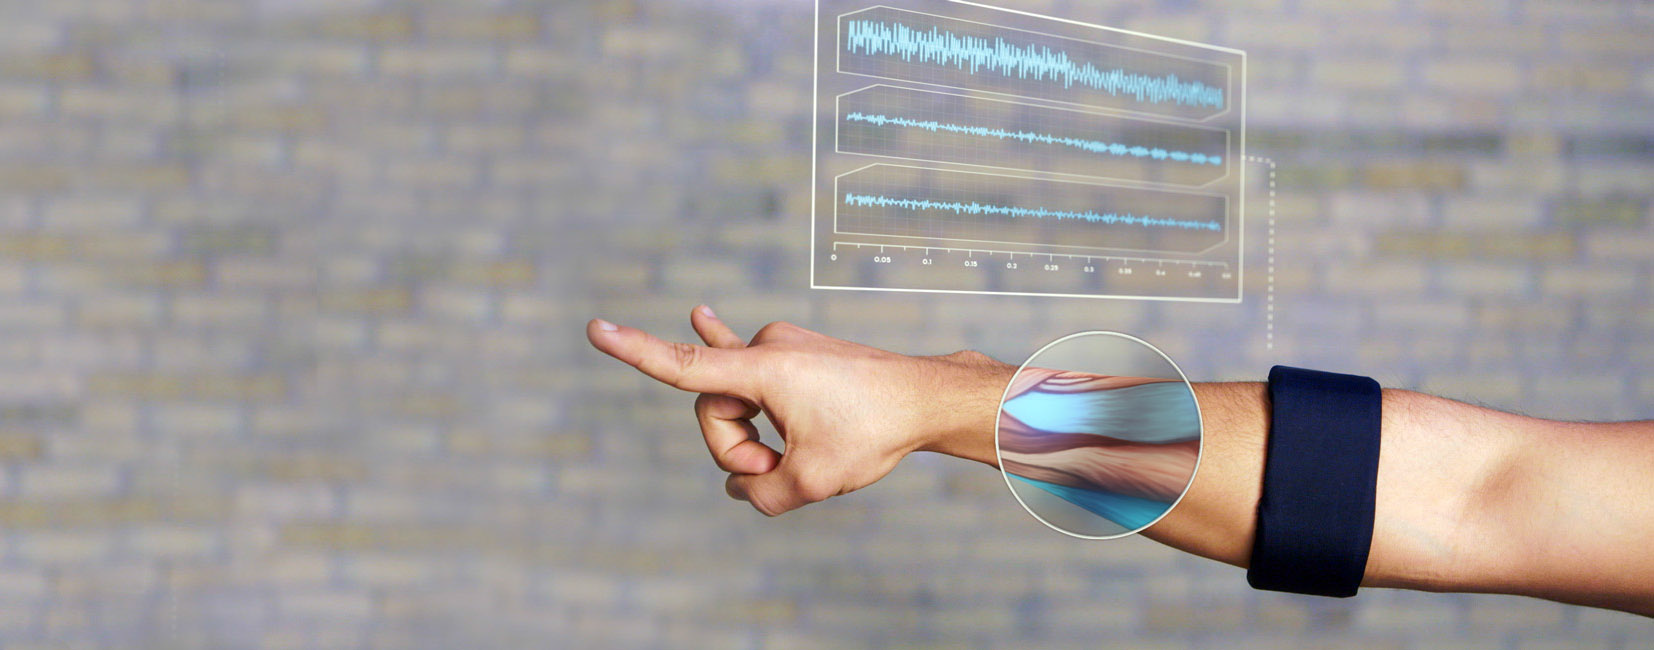
\includegraphics[width=15cm,left,keepaspectratio]{figures/myo}
\caption{Myo armband}
\label{myo}
\end{figure}
Myo uses five gestures to interact with the environment shown in Fig \ref{motions}, these five gestures include fist, double tap, finger spread, wave left and wave right. 
\begin{figure}[H]
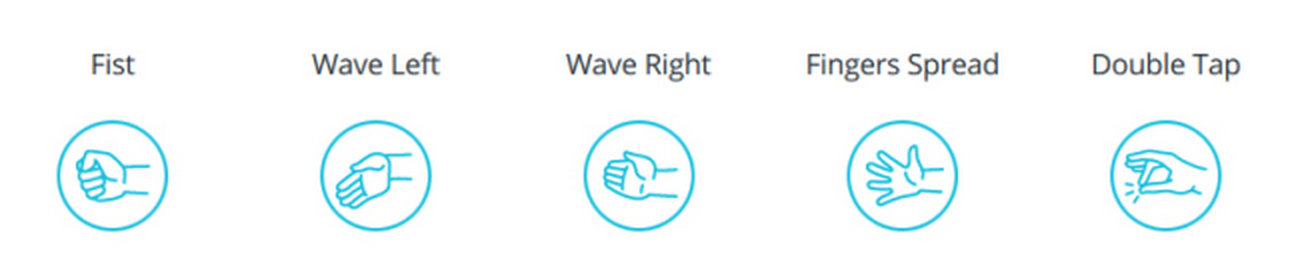
\includegraphics[width=15cm,left,keepaspectratio]{figures/motions}
\caption{Gestures recognized by Myo}
\label{motions}
\end{figure}
Myo's sampling frequency is 200 Hz that means that it provides 200 EMG samples per second. Therefore, frequencies up to Nyquist frequency of 100 Hz can be detected. When the Bluetooth connection is set up the users are able to map each gesture into a particular input event in order to interact and communicate with the connected devices. 

\section{IMU of the Myo Armband}
Although we will not use in this work the offered IMU data. The inertial measurement unit consists of multiple single sensors in order to acquire accelerometer, gyroscope and orientation data. The IMU sensors are contained in the fourth pod as in Fig. \ref{myo_enum}, where also the Bluetooth, the Universal Serial Bus (USB) and two LEDs find place. The sampling frequency for the IMU data is determined at 50 Hz \cite{IMU}.\\
The accelerometers in the Myo armband measures the acceleration of the forearm. With the help of accelerometers and the provided framework of Thalmic Labs, Myo can detect not only the basic movements of the hand but also more complex movements.\\
The gyroscopes helps to track the change in the orientation while the armband is rotated and translated by the user's arm. The way the gyroscopes works is that it simulates an artificial horizon and maintains orientation according to that horizon. The gyroscope provides the user with angular velocity data, which is provided in vector format. \\
Last but not least, the orientation data indicates which way the Myo armband is pointed in terms of roll, pitch and yaw. The orientation data is delivered in two possible formats: angle-velocity and quaternions.

\begin{figure}[h!]
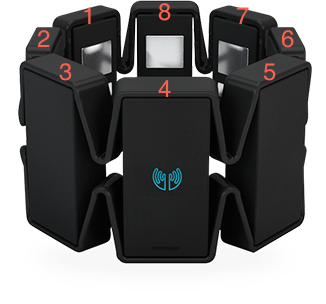
\includegraphics[width=7cm,center,keepaspectratio]{figures/myo_enum}
\caption{EMG channel assignments}
\label{myo_enum}
\end{figure}

\section{Gesture Recognition} 
Gesture recognition can be seen as a way for computers to understand body language. The aforementioned supported gestures can help the user to interact with technology but it is restrictive as it limits the total recognized gestures down to five. However, the experienced user can have access to the IMU and EMG data and develop his/her own ideas to recognize custom gestures such as flexion and extension of each individual finger. In this current work, we will use one Myo which we wear in the right arm and fetch EMG signals with it. The arm during all experiments will remain still. Therefore, the IMU data are not needed for this study. The reason for not moving the whole arm, is that we want to study only the individual movements of the fingers with Myo's EMG sensors.

\section{Armband positioning}
Myo's position on the user's arm is very important. From that, it depends which sensor is recording which muscle. If we change the position of the sensors during the experiment the values of each of the eight channels will give us different results and we will have not sensible data. Therefore, during the experiment the sensors must be set firmly on the user's arm. Furthermore, during the whole sequence of experiments the Myo must be worn in the same approximately position as best as possible in order to have a homogeny of results for each channel from each experiment. In the current work, the subject will wear the Myo on top of the right hand after strecthing his/her hand with the back of the hand facing downwards and placing the pod with LED indicator to face towards the wrist. 
\begin{figure}[H]
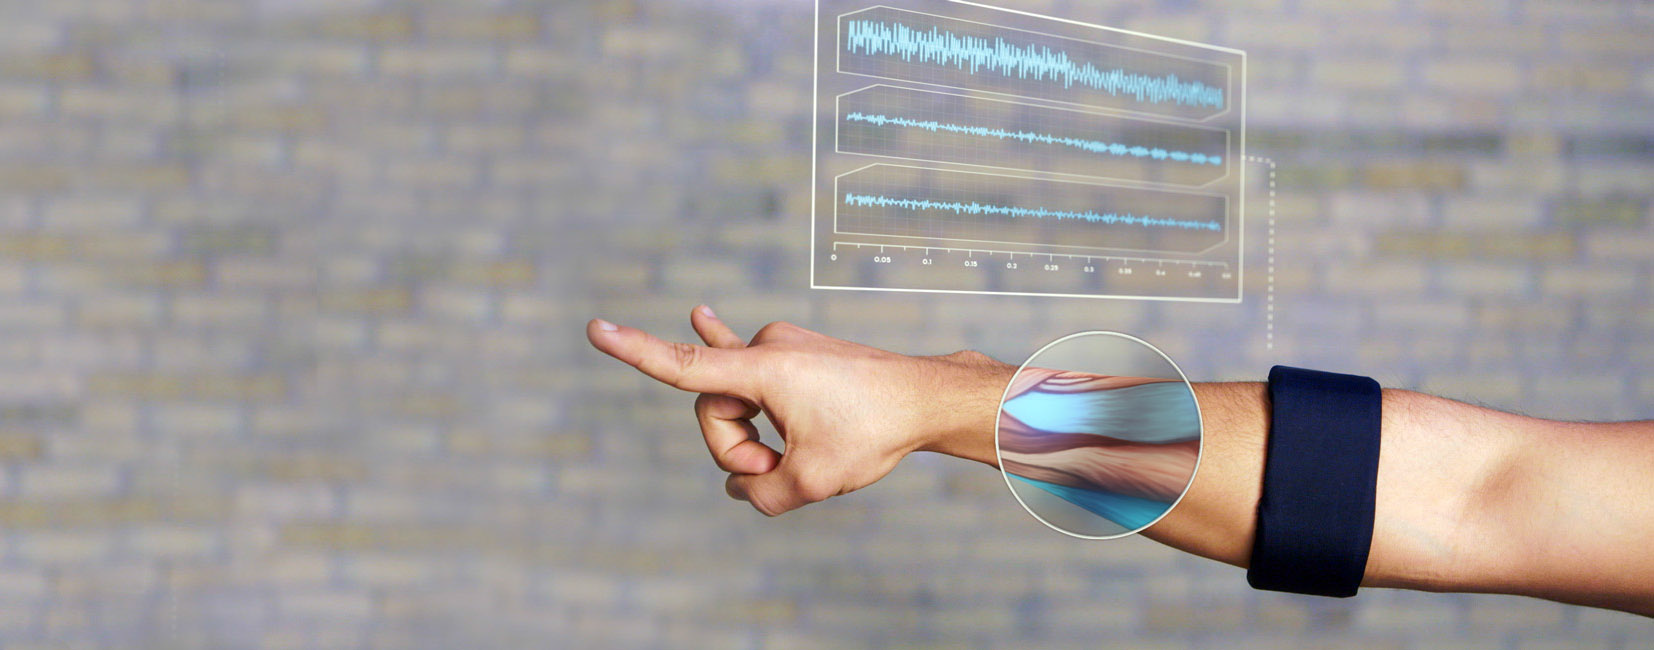
\includegraphics[width=15cm,left,keepaspectratio]{figures/myo}
\caption{Positioning of Myo in user's forearm. \cite{fig:myo_on_armband} }
\label{fig:myo_on_armband}
\end{figure}